\section{决策部分}
\label{sec:policy}
\begin{frame}{决策部分}
    \begin{itemize}
        \item 输入:语义地图 (semantic map)
        \item 输出:
            \begin{itemize}
                \item 长期目标 (long-term goal)
                \item 当前行动 (action, path)
                \begin{itemize}
                    \item $a_t$: 向前,左转,右转,停
                \end{itemize}
            \end{itemize}
    \end{itemize}
    \note{
        \begin{itemize}
            \item 决策部分负责接受感知部分输出的语义地图,并分成两步完成决策
            \item 第一步全局决策:选择一个long-term goal,表示在未来的一段时间内目标到达的位置
            \item 第二步局部决策:决定为了到达long-term goal,应该如何行动
        \end{itemize}
    }
\end{frame}


\begin{frame}{决策部分总体结构}
    \centering
    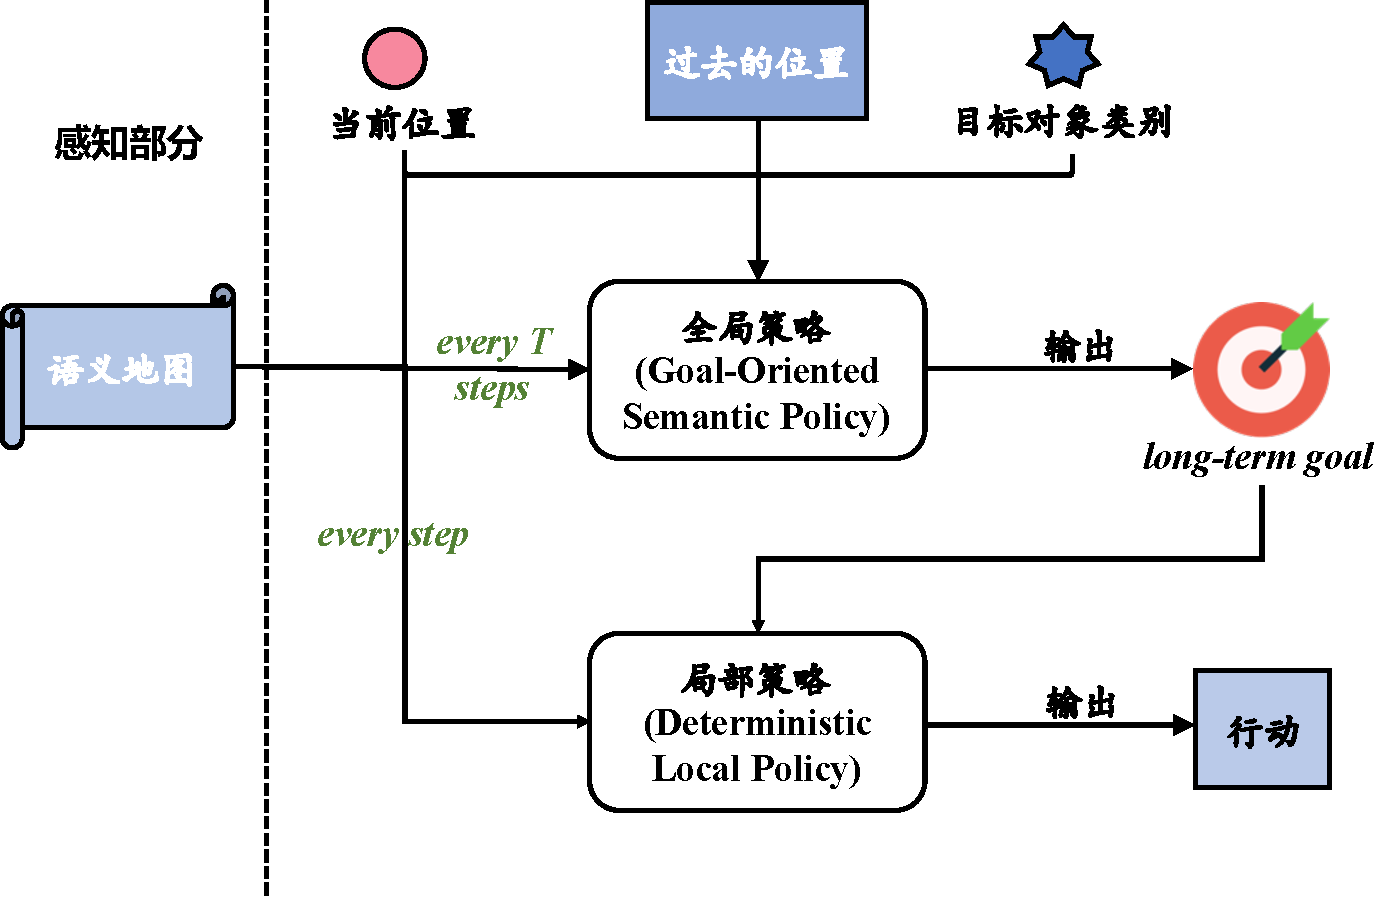
\includegraphics[width=11cm]{assets/policy_structure.pdf}
    \note{
        决策部分可以大致分为两个部分:全局决策和局部决策
        \begin{itemize}
            \item 全局决策:得到长期目标 (\emph{long-term goal})
                \begin{itemize}
                    \item 输入:带有预测信息的语义地图,语义目标
                    \item coarse time scale: 每T步更新一次long-term goal(减少复杂度)
                    \item 使用监督训练模型(神经网络),进一步获取语义先验知识
                    \item 决策接下来T步局部决策的目标到达位置
                \end{itemize}
            \item 局部决策:得到抵达long-term goal的路径 (path)
                \begin{itemize}
                    \item 输入:语义地图,当前位置,long-term goal
                    \item 也就知道了当前应该采取的行动$a_t$
                    \item fine time scale: 每一步都需要决策
                    \item 采用Far Marching Method~\cite*{...}
                \end{itemize}
        \end{itemize}
    }
\end{frame}

\begin{frame}{局部决策}
    对于局部决策,我们参考~\cite*{chaplot2020object},采用Far Marching Method:
    \begin{itemize}
        \item 利用语义地图中的obstacle channel即可
        \item 
    \end{itemize}
\end{frame}

\begin{frame}{全局决策}
    \centering
    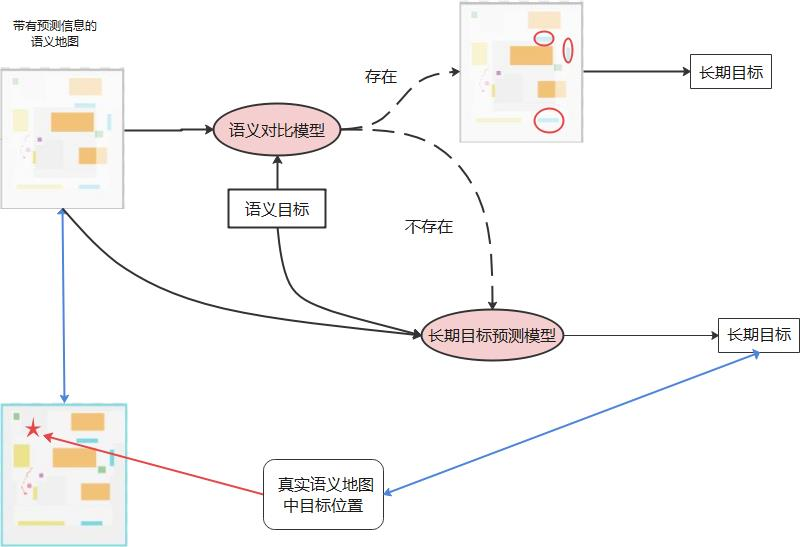
\includegraphics[width=11cm]{assets/global_policy.png}
    \note{
        %\footnotesize
        对于全局决策,我们处理了两种可能的情况:
        \begin{itemize}
        \item case1: 预测语义地图中存在语义目标;
        \item case2: 预测语义地图中不存在语义目标
        \end{itemize} }
\end{frame}

\begin{frame}{全局决策-case1}
         预测语义地图中存在语义目标时:\\直接通过对比输出语义目标位置作为长期目标(可能存在多个)
\end{frame}

\begin{frame}{全局决策-case2}
     预测语义地图中不存在语义目标时:
              \begin{itemize}
                  %\footnotesize
                  \item 采用监督模型预测可能的一个长期目标位置。
                  \item 输入:预测语义地图,语义目标; 输出:长期目标位置。
                  \item 真相目标位置的获取:与感知任务部分所讲类似,使用模拟器或环境绘制提供的全部语义地图以及语义分割对比技术确定。
                  \item 与我们参考的论文[16]相比,采用监督学习进一步探索语义先验,期望会获得更好地收敛速度和更准确的结果。
                  \item 为提高效率,降低复杂度,采用粗粒度时间预测(经过T步行动进行一次长期目标的选择)。(T可参考论文[16]使用25)。
                  \item 模型可进一步采用输入当前位置以及前一时刻位置,用距最近目标物体的距离变化作为reward进行强化学习。
              \end{itemize}
\end{frame}